\begin{frame}{Análisis exploratorio de datos. Audio.\newline Dominio de la Frecuencia}
	\begin{columns}
		\begin{column}{0.5\textwidth}
			\begin{figure}
				\centering
				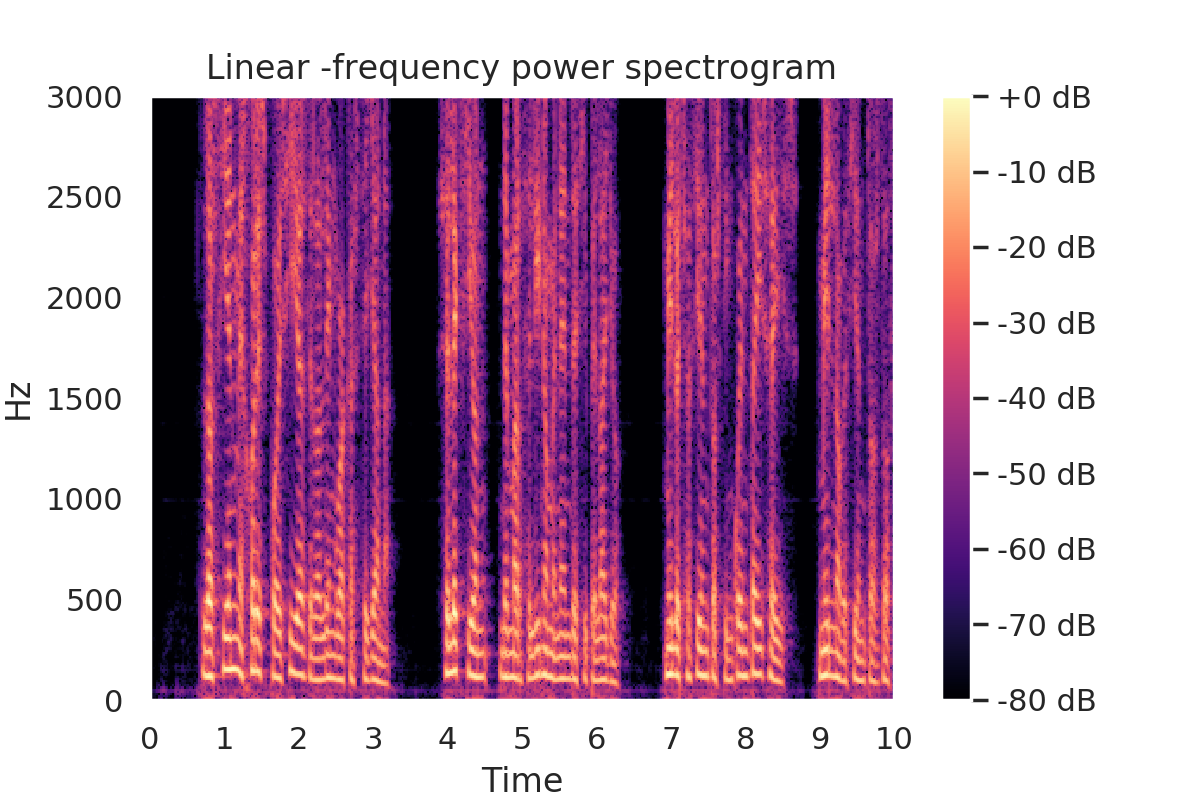
\includegraphics[width=0.9\columnwidth]{../figures/audio_book_spectrogram.png}
				\vspace*{-5pt}
				\caption{Espectrograma de la voz humana}
				\label{fig: voice_spectral}
			\end{figure}
			\vspace*{-20pt}
			\begin{figure}
				\centering
				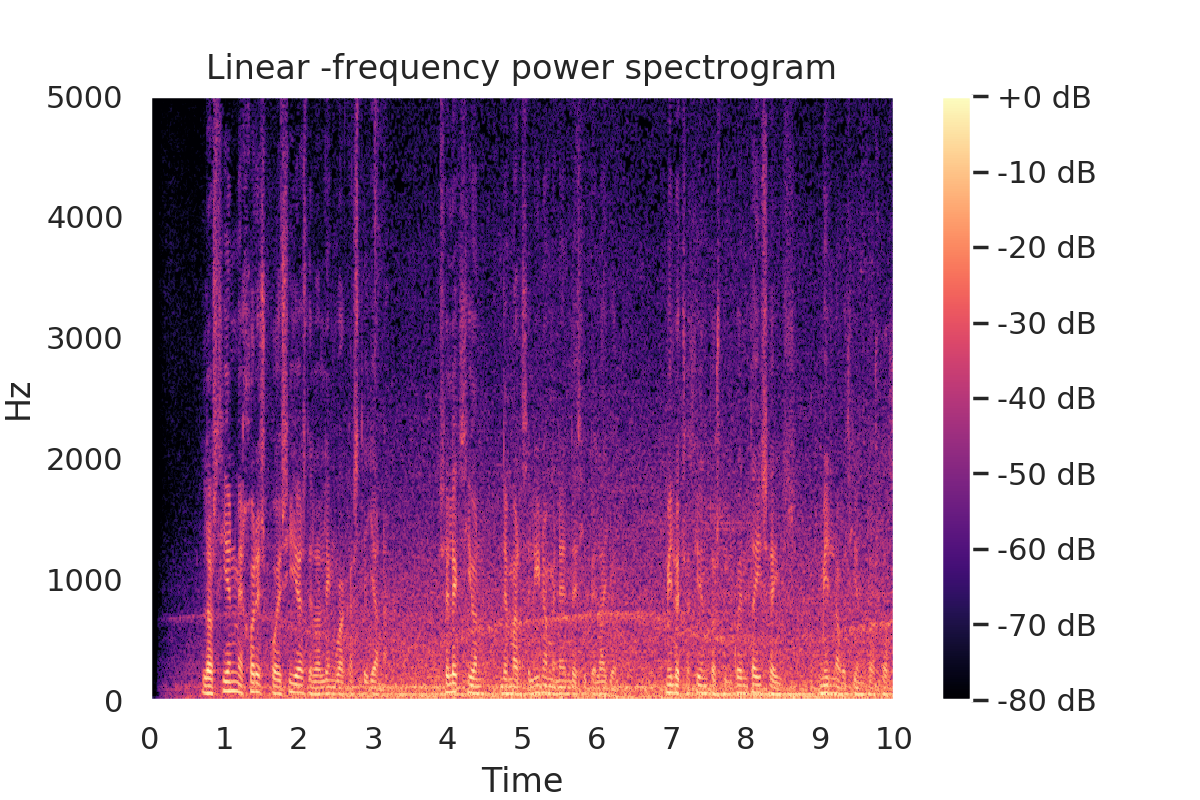
\includegraphics[width=0.9\columnwidth]{../figures/combination_spectrogram.png}
				\vspace*{-5pt}
				\caption{Espectrograma de las pistas combinadas}
				\label{fig: combination_spectral}
			\end{figure}
		\end{column}
		\begin{column}[t]{0.5\textwidth}
			\vspace*{-113pt}
			\begin{figure}
				\centering
				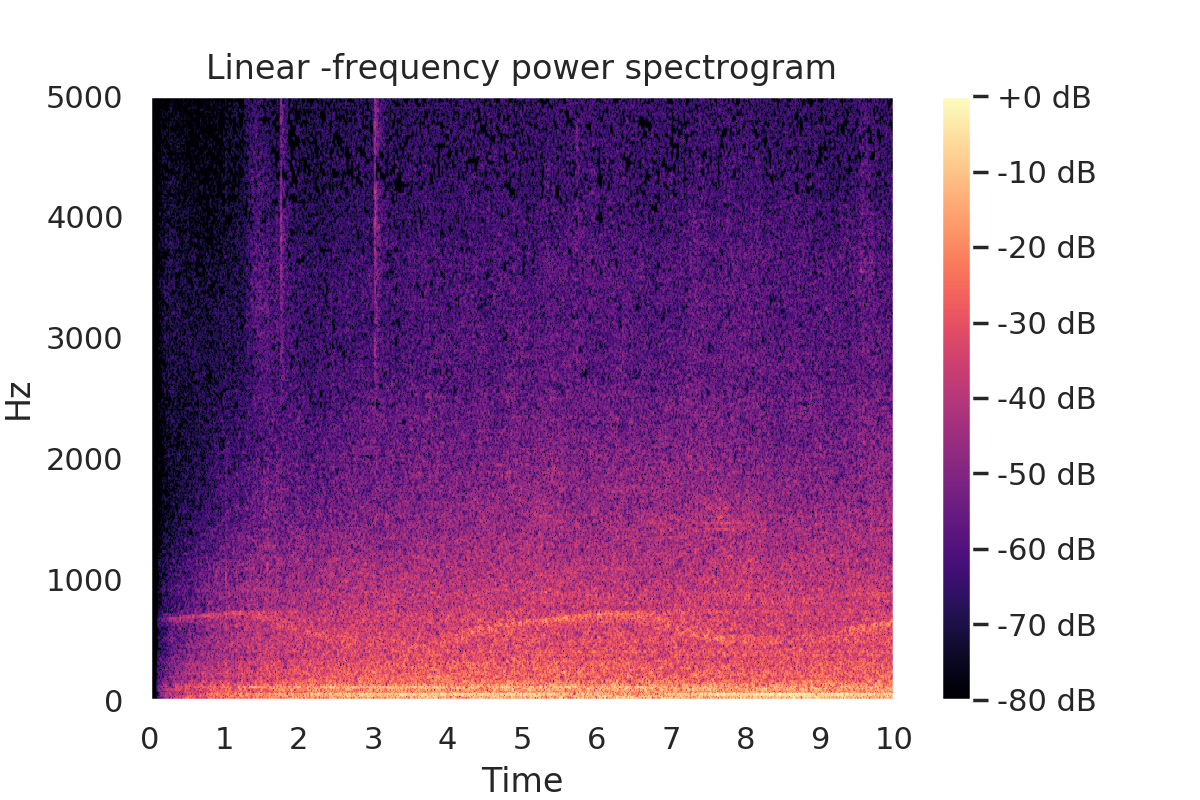
\includegraphics[width=0.9\columnwidth]{../figures/noise_spectrogram.png}
				\vspace*{-5pt}
				\caption{Espectrograma del ruido}
				\label{fig: noise_spectral}
			\end{figure}
			\begin{figure}
				\centering
				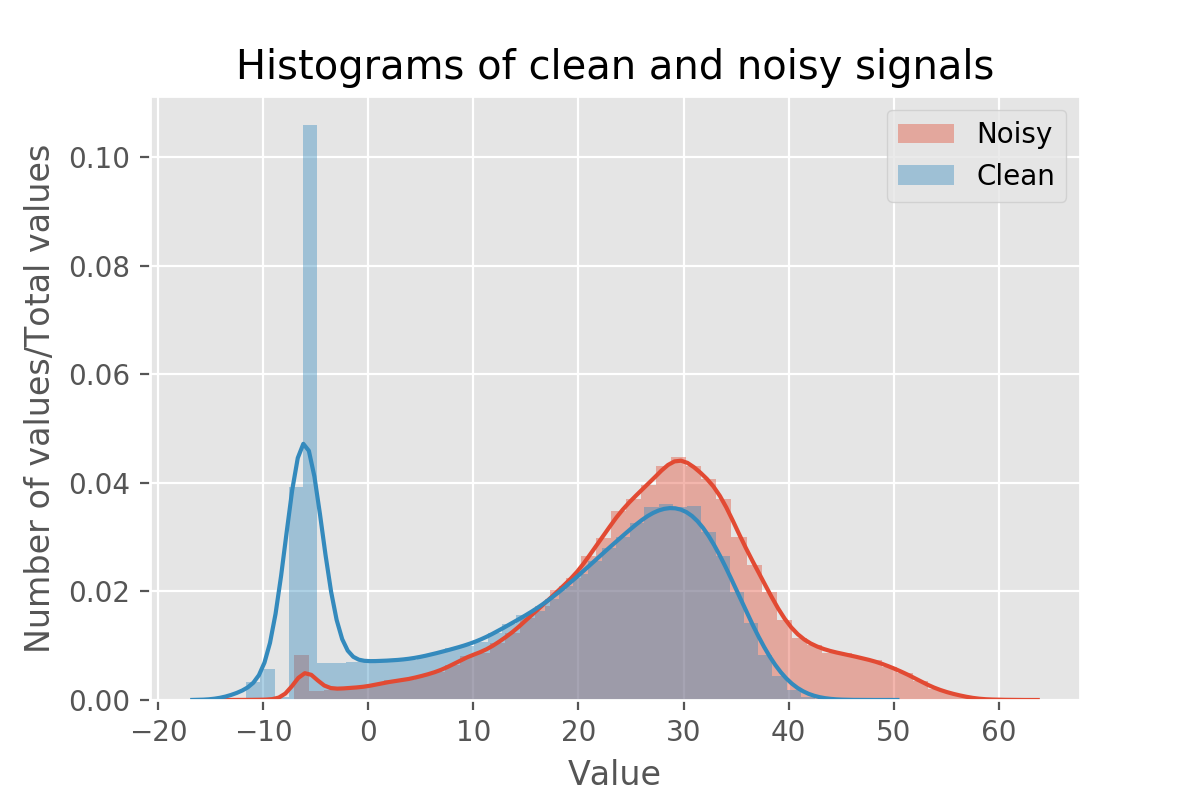
\includegraphics[width=0.6\columnwidth]{../figures/band0_clean_noisy_hist.png}
				\caption{Espectrograma de las pistas combinadas}
				\label{fig: band0_clean_noisy_hist}
			\end{figure}
		\end{column}
	\end{columns}
\end{frame}
\begin{frame}{Análisis exploratorio de datos. Audio.\newline Dominio del Tiempo}
	\vspace*{-2pt}
	\begin{figure}
		\centering
		\begin{subfigure}[t]{0.5\textwidth}
			\centering
			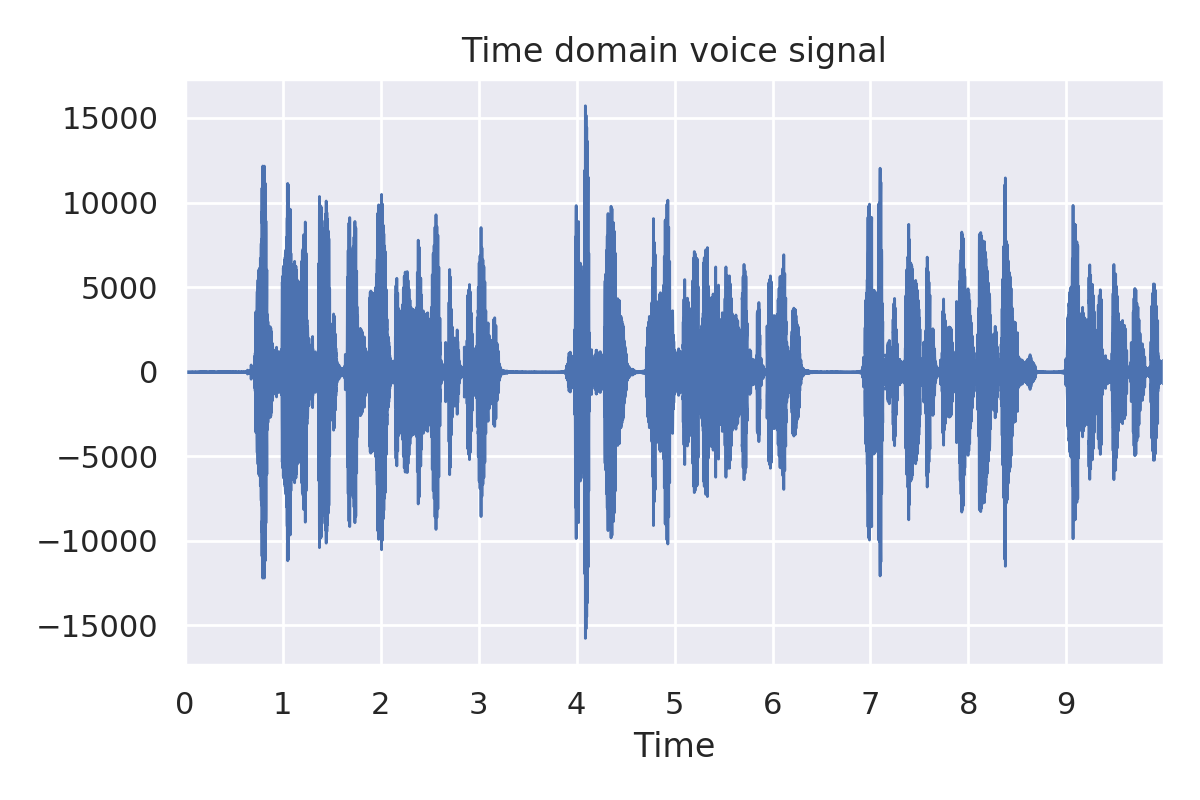
\includegraphics[width=0.9\columnwidth]{../figures/audio_book_time.png}
			\vspace*{-5pt}
			\caption{Forma de la señal de audio en el dominio del tiempo}
			\label{fig: voice_time}
		\end{subfigure}%
		\hspace*{10pt}
		\begin{subfigure}[t]{0.5\textwidth}
			\centering
			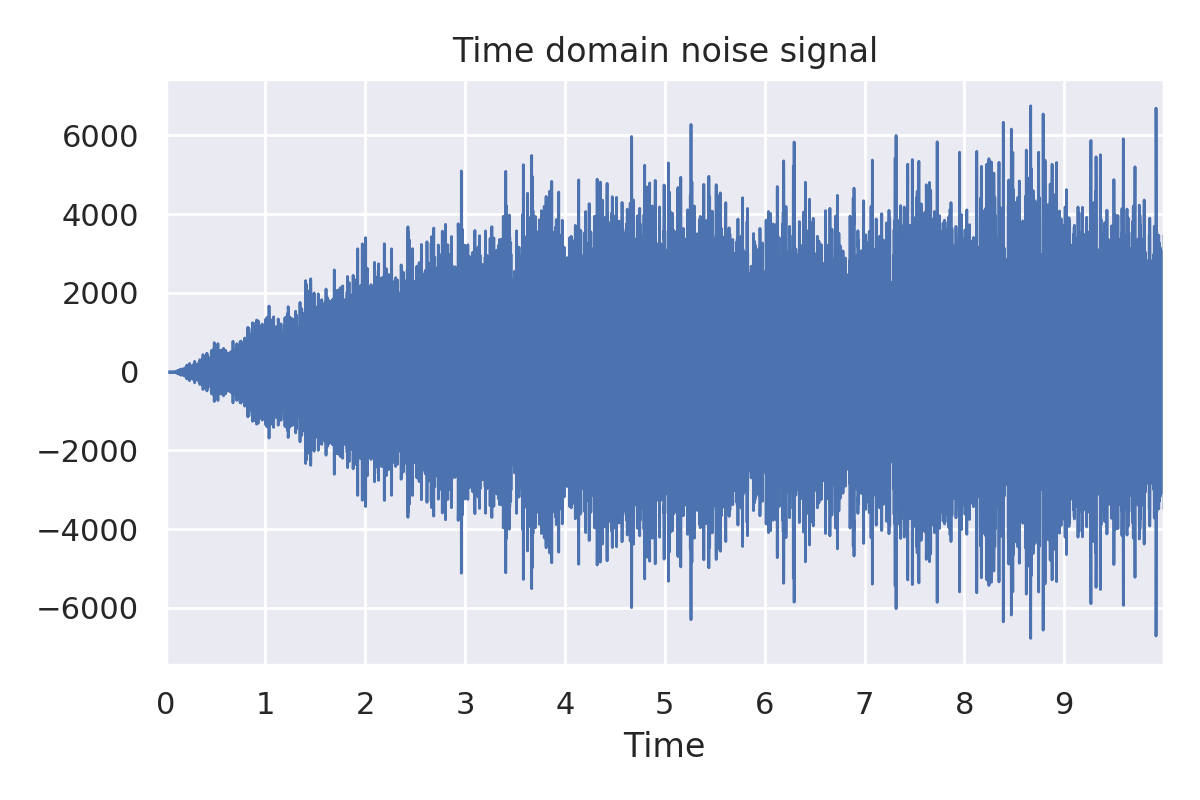
\includegraphics[width=0.9\columnwidth]{../figures/noise_time.png}
			\vspace*{-5pt}
			\caption{Forma de la señal de ruido en el dominio del tiempo}
			\label{fig: noise_time}
		\end{subfigure}
	\end{figure}
	\vspace*{-15pt}
	\begin{figure}
		\centering
		\begin{subfigure}[t]{0.5\textwidth}
			\centering
			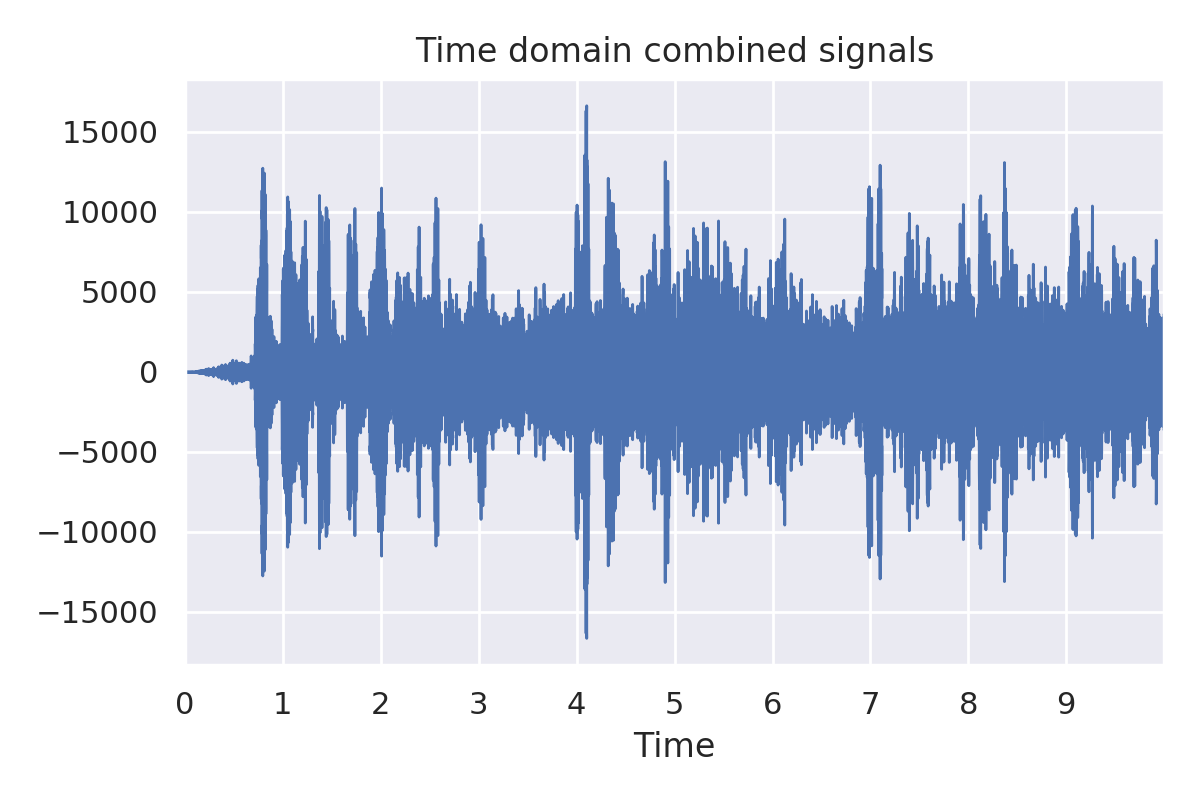
\includegraphics[width=\columnwidth]{../figures/combination_time.png}
			\vspace*{-10pt}
			\caption{Forma de la señal combinada de audio y ruido en el dominio del tiempo}
			\label{fig: combination_time}
		\end{subfigure}%
		\hspace*{10pt}
		\begin{subfigure}[t]{0.5\textwidth}
			\centering
			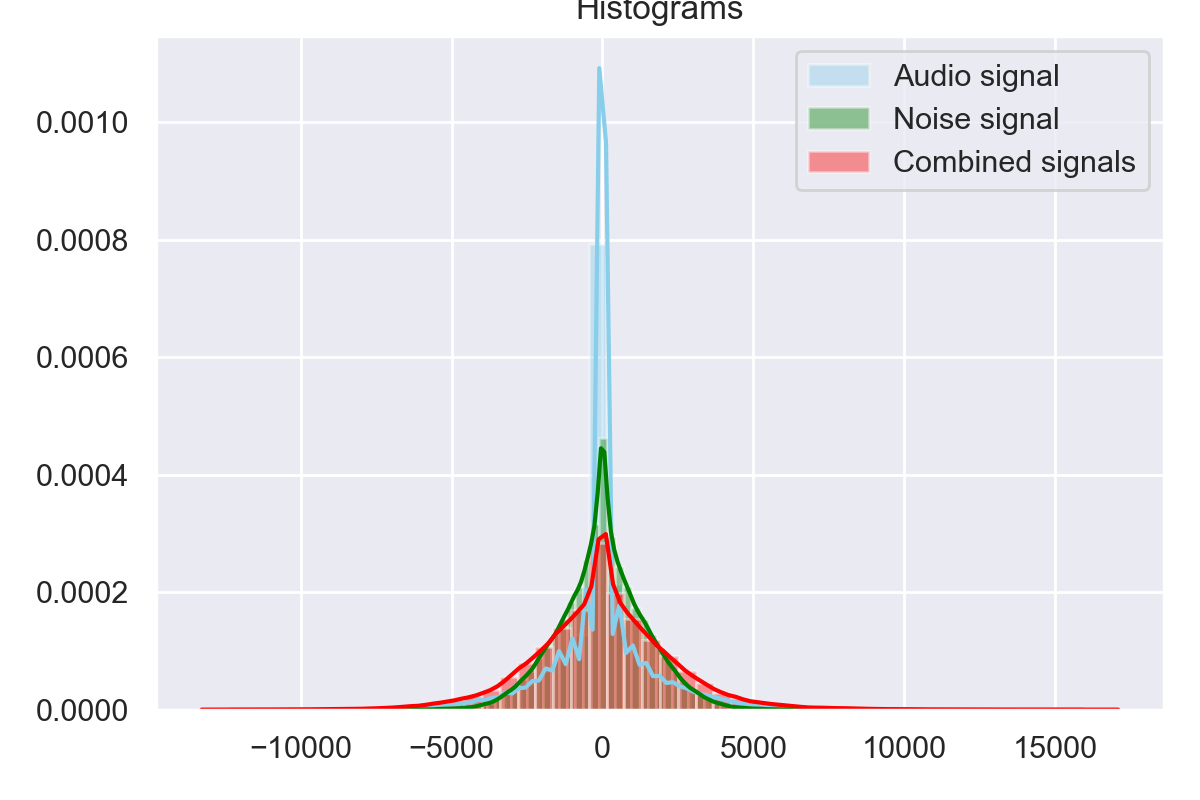
\includegraphics[width=\columnwidth]{../figures/hist_time.png}
			\vspace*{-10pt}
			\caption{Histogramas superpuestos de las tres señales}
			\label{fig: hist_time}
		\end{subfigure}
	\end{figure}
\end{frame}
\begin{frame}{Análisis exploratorio de datos. Audio.\newline Conclusiones}
	\begin{itemize}
		\item \textbf{La voz humana no es continua en el tiempo} (la persona se para para respirar mientras habla) lo que crea un espectro seccionado en el tiempo. Por el contrario el \textbf{ruido sí es continuo en el tiempo}.
		\vspace{10pt}
		\item El \textbf{espectro de la voz humana está acotado en frecuencia} mientras que el espectro del ruido, en general, no. Como implicación directa tiene que para analizar el audio en el dominio de la frecuencia se puede acotar la tasa de muestreo a la banda donde la voz humana se encuentra, ahorrando mucho procesado.
		\vspace{10pt}
		\item La \textbf{voz humana} se caracteriza por tener unas \textbf{frecuencias características} que varían en el tiempo y están relacionadas entre sí (tono fundamental y armónicos). Por el contrario el ruido, no presenta relación entre sus componentes espectrales.
		\vspace{10pt}
		\item Tras la combinación de los audios, si las amplitudes del ruido no son lo suficientemente grandes, las componentes frecuenciales de la voz siguen siendo predominantes.
	\end{itemize}
\end{frame}